
%(BEGIN_QUESTION)
% Copyright 2006, Tony R. Kuphaldt, released under the Creative Commons Attribution License (v 1.0)
% This means you may do almost anything with this work of mine, so long as you give me proper credit

Determine the temperature of the measurement junction in this thermocouple circuit (type K), given the reference junction temperatures and the voltmeter indications.  Round your answer to the nearest whole degree Fahrenheit:

$$\includegraphics[width=15.5cm]{i00382x01.eps}$$

\begin{itemize}
\item{} $T_{reference}$ = 70$^{o}$ F ; Voltmeter voltage = 20.018 mV ; $T_{measurement}$ = ??? 
\item{} $T_{reference}$ = 65$^{o}$ F ; Voltmeter voltage = 5.833 mV ; $T_{measurement}$ = ??? 
\item{} $T_{reference}$ = 52$^{o}$ F ; Voltmeter voltage = 31.420 mV ; $T_{measurement}$ = ??? 
\item{} $T_{reference}$ = 73$^{o}$ F ; Voltmeter voltage = $-$2.027 mV; $T_{measurement}$ = ??? 
\end{itemize}

\vskip 20pt \vbox{\hrule \hbox{\strut \vrule{} {\bf Suggestions for Socratic discussion} \vrule} \hrule}

\begin{itemize}
\item{} With RTDs, it is possible to use a {\it formula} to relate resistance with temperature rather than having to consult a table.  Do you think this is possible for thermocouples as well?  If so, what do you think the voltage/temperature formula describing a thermocouple might look like?
\end{itemize}

\underbar{file i00382}
%(END_QUESTION)





%(BEGIN_ANSWER)

\noindent
{\bf Partial answer:}

\begin{itemize}
\item{} $T_{reference}$ = 70$^{o}$ F ; Voltmeter voltage = 20.018 mV ; $T_{measurement}$ = 941 $^{o}$F 
\item{} $T_{reference}$ = 73$^{o}$ F ; Voltmeter voltage = $-$2.027 mV; $T_{measurement}$ = $-$20 $^{o}$F 
\end{itemize}

%(END_ANSWER)





%(BEGIN_NOTES)

(From ITS-90 thermocouple table:)

\begin{itemize}
\item{} $T_{ref}$ = 70$^{o}$ F ($V_{ref}$ = 0.843 mV); $V_{meter}$ = 20.018 mV ; {\bf $T_{meas}$ = 941$^{o}$ F ($V_{meas}$ = 20.861 mV)}
\item{} $T_{ref}$ = 65$^{o}$ F ($V_{ref}$ = 0.731 mV) ; $V_{meter}$ = 5.833 mV ; {\bf $T_{meas}$ = 321$^{o}$ F ($V_{meas}$ = 6.564 mV)}
\item{} $T_{ref}$ = 52$^{o}$ F ($V_{ref}$ = 0.441 mV); $V_{meter}$ = 31.420 mV ; {\bf $T_{meas}$ = 1410$^{o}$ F ($V_{meas}$ = 31.861 mV)}
\item{} $T_{ref}$ = 73$^{o}$ F ($V_{ref}$ = 0.910 mV) ; $V_{meter}$ = $-$2.027 mV; {\bf $T_{meas}$ = $-$20$^{o}$ F ($V_{meas}$ = $-$1.117 mV)}
\end{itemize}







\vfil \eject

\noindent
{\bf Summary Quiz:}

Referencing a thermocouple table (ITS-90), determine the temperature of a type J thermocouple (measurement junction) assuming the voltmeter reads 14.843 millivolts and the ambient temperature where the voltmeter leads connect to the thermocouple wires is 64 $^{o}$F:

\begin{itemize}
\item{} 524 $^{o}$F
\vskip 5pt 
\item{} 493 $^{o}$F
\vskip 5pt 
\item{} 553 $^{o}$F 
\vskip 5pt 
\item{} 479 $^{o}$F
\vskip 5pt 
\item{} 494 $^{o}$F
\vskip 5pt 
\item{} 555 $^{o}$F
\end{itemize}


%INDEX% Measurement, temperature: thermocouple

%(END_NOTES)


